\textbf{2.1.} 如习题 2.1 图所示的两块大小相同的平行金属板, 所带的电量 $Q_{1}$ 和 $Q_{2}$ 不相等, 若 $Q_{1} > Q_{2}$ , 略去边缘效应.

(1) 证明: 相向的两面上电荷的面密度的大小相等而符号相反, 相背的两面上电荷的面密度大小相等而符号相同.

(2) 计算金属板各面的电量.

\begin{center}
    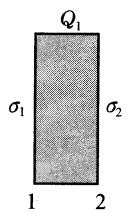
\includegraphics[width=0.1\linewidth]{figures/fig_2_2_1.jpg}
    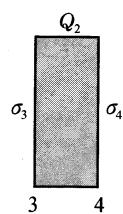
\includegraphics[width=0.1\linewidth]{figures/fig_2_2_2.jpg}
\end{center}

\vfill

\textbf{2.2.} 如习题 2.2 图所示, 半径为 $R_{1}$ 的导体球外有同心的导体球壳, 壳的内外半径分别为 $R_{2}$ 和 $R_{3}$ , 已知球壳带的电量为 Q, 内球的电势为零. 求内球的电荷量和球壳的电势.

\begin{center}
    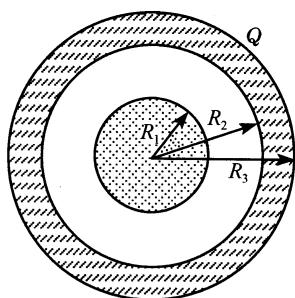
\includegraphics[width=0.2\linewidth]{figures/fig_2_2_3.jpg}
\end{center}

\vfill

\newpage

\textbf{2.3.} 一肥皂泡的半径为 $r$ , 肥皂水的表面张力系数为 $\alpha$ , 外部空气的压强为 $p$ . 使这肥皂泡带上电荷 $Q$ 后, 半径增大为 $R$ , 证明

$$
(R ^ {3} - r ^ {3}) p + 4 \alpha (R ^ {2} - r ^ {2}) = \frac {Q ^ {2}}{3 2 \pi^ {2} \varepsilon_ {0} R}
$$

\vfill

\textbf{2.4.} 有若干个互相绝缘的不带电的导体 $A, B, C, \cdots$ , 它们的电势都是零, 如果使其中任一个导体例如 $A$ 带上正电, 证明:

(1) 所有这些导体的电势都高于零;

(2) 其他导体的电势都低于 $A$ 的电势.

\vfill

\newpage

\textbf{2.5.} 如习题 2.5 图所示, 在金属球 A 内有两个球形空腔, 此金属球整体上不带电, 在两空腔中心各放置一点电荷 $q_{1}$ 和 $q_{2}$ , 在金属球 A 之外远处放置一点电荷 q (q 至 A 中心距离 r >> 球 A 的半径 R). 计算作用在 A、 $q_{1}$ 、 $q_{2}$ 、q 四物体上的静电力.

\begin{center}
    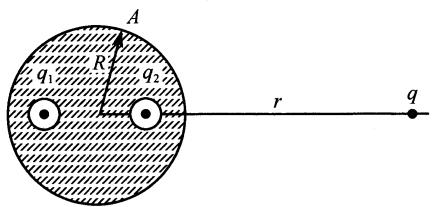
\includegraphics[width=0.3\linewidth]{figures/fig_2_6_1.jpg}
\end{center}

\vfill

\textbf{2.6.} 一电容器由三片面积都是 $6.0\mathrm{cm}^2$ 的锡箔构成，相邻两箔间的距离都是 $0.10\mathrm{mm}$ ，外边两箔片联在一起构成为一极，中间箔片作为另一极，如习题2.6图所示。

(1) 求电容 C;

(2) 若在这电容器上加 220V 的电压, 外箔片电势高于中间箔片, 问外箔片和中间箔片上的面电荷密度各是多少?

\begin{center}
    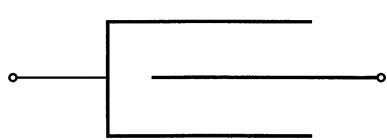
\includegraphics[width=0.3\linewidth]{figures/fig_2_6_2.jpg}
\end{center}

\vfill

\newpage

\textbf{2.7.} 如习题 2.7 图所示,一平行板电容器中间插入一厚度为 t 的导体板,导体板的面积为电容器极板面积的一半.求插入后的电容值.

\begin{center}
    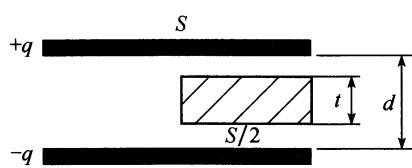
\includegraphics[width=0.3\linewidth]{figures/fig_2_8.jpg}
\end{center}
\vfill

\textbf{2.8.} 有5个电容器,如习题2.8图所示方式连接, $C_{1}=C_{5}=2\mu F,C_{2}=C_{3}=C_{4}=1\mu F$ ,并接到电压为U=600V的电源上,求每个电容器上的电压值.
\begin{center}
    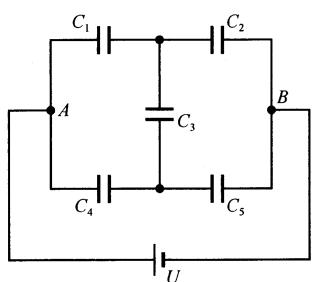
\includegraphics[width=0.25\linewidth]{figures/fig_2_9_1.jpg}
\end{center}

\vfill

\newpage

\textbf{2.9.} 如习题 2.9 图所示, 三个共轴的金属圆筒, 长度都是 $l$ ，半径分别为 $a, b$ 和 $d$ ，里外两筒用导线联在一起作为一极，中间圆筒作为另一极。略去边缘效应。求电容C.

\begin{center}
    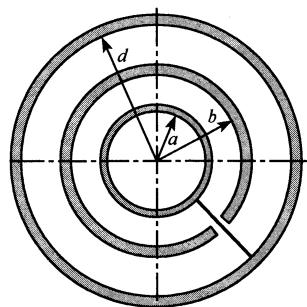
\includegraphics[width=0.25\linewidth]{figures/fig_2_9_2.jpg}
\end{center}

\vfill

\textbf{2.10.} 在 $100^{\circ}$ C 和 1.0atm 时，饱和水蒸气的密度为 $598g \cdot m^{-3}$ ，水的相对分子质量为 18，水分子的电偶极矩为 $6.2 \times 10^{-30} C \cdot m$ . 求这时水蒸气电极化强度的最大值.

\vfill

\newpage

\textbf{2.11.} 电介质强度是指电介质能经受的最大电场强度而不被击穿,迄今所知道的电介质强度的最大值约为 $1 \times 10^{9} \mathrm{~V} \cdot \mathrm{m}^{-1}$ . 试问:

(1) 当金属导体处在这种介质中时, 它的面电荷密度 $\sigma$ 最大不能超过多少?

(2) 金属导体中原子的直径约为 $2 \times 10^{-10}$ m，金属导体表面一层原子中，缺少或多出一个电子的原子数最多不能超过百分之几？

\vfill

\textbf{2.12.} 如习题 2.12 图所示,一平行板电容器两极板的面积都是 $2.0 \mathrm{~m}^{2}$ , 相距为 $5.0 \mathrm{~mm}$ . 两板加上 $10^{4} \mathrm{~V}$ 电压后, 撤去电源, 再在其间填满两层均匀介质, 一层厚 $2.0 \mathrm{~mm}$ , 相对介电常量为 $\varepsilon_{\mathrm{r} 1} = \varepsilon_{1} / \varepsilon_{0} = 5.0$ ; 另一层厚 $3.0 \mathrm{~mm}, \varepsilon_{\mathrm{r} 2} = \varepsilon_{2} / \varepsilon_{0} = 2.0$ . 略去边缘效应.

(1) 求各介质中电极化强度 $P$ 的大小;

(2) 当电容器紧靠介质 2 的极板接地 (即电势为零) 时, 另一极板 (正极板) 的电势是多少? 两介质接触面上的电势是多少?
\begin{center}
    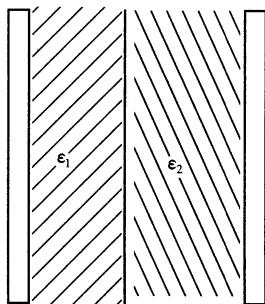
\includegraphics[width=0.2\linewidth]{figures/fig_2_12.jpg}
\end{center}

\vfill

\newpage

\textbf{2.13.} 圆柱电容器是由半径为 $R_{1}$ 的直导线和与它同轴的导体圆筒构成，圆筒内半径为 $R_{2}$ ，长为 $l$ ，其间充满了介电常量为 $\varepsilon$ 的介质。设沿轴线单位长度上，导线带电量为 $\lambda_{0}$ ，圆筒带电量为 $-\lambda_{0}$ 。略去边缘效应，求：

（1）介质中的电场强度 $E$ 、电位移矢量 $D$ 、极化强度 $P$ 、极化电荷体密度 $\rho'$ 和介质表面的极化电荷面密度 $\sigma'$ ；

（2）两极板的电势差 $U$ ；

（3）电容 $C$ 。

\vfill

\textbf{2.14.} 半径为 $a, b (a < b)$ 的同心导体球壳之间充满非均匀介质，介电常量为 $\varepsilon = \varepsilon_0 / (1 + kr)$ ，其中 $k$ 为常数， $r$ 为径向距离。内球壳表面有电荷 $Q$ ，外球壳接地。计算

(1) 系统的电容；

(2) 介质内的极化电荷密度；

(3) 球面上极化电荷面密度。

\vfill

\newpage

\textbf{2.15.} 有一半径为 $R$ 的金属球, 外面包有一层相对介电常量为 $\varepsilon_{\mathrm{r}} = 2$ 的均匀电介质, 壳内外半径分别为 $R$ 和 $2R$ , 介质内均匀分布着电量为 $q_{0}$ 的自由电荷, 金属球接地. 求介质球壳外表面的电势.

\vfill

\textbf{2.16.} 平行板电容器两极板相距 3.0cm, 其间放有一层相对介电常量为 $\varepsilon_{r}=2$ 的介质, 位置与厚度如习题 2.16 图所示. 已知极板上面电荷密度为 $\sigma=8.85\times10^{-10}C\cdot m^{-2}$ , 略去边缘效应, 求:

(1) 极板间各处 P、E 和 D 的值;

(2) 极板间各处的电势(设 A 板的电势 $V_{A}=0$ ).

\begin{center}
    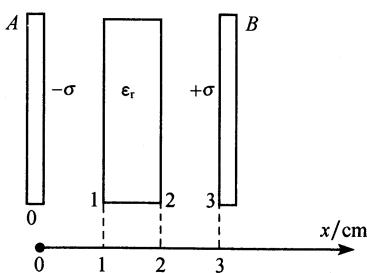
\includegraphics[width=0.3\linewidth]{figures/fig_2_17.jpg}
\end{center}

\vfill

\newpage

\textbf{2.17.} 球形电容器由半径为 $R_{1}$ 的导体和与它同心的导体球壳构成，壳的内半径为 $R_{2}$ ，其间有两层均匀介质,分界面的半径为 r, 内、外层介质的介电常量分别为 $\varepsilon_{1}$ 和 $\varepsilon_{2}$ .

(1) 求电容 C;

(2) 当内球带电荷—Q 时, 求介质表面上极化电荷的面密度.


\vfill

\textbf{2.18.} 两介电常量分别为 $\varepsilon_{1}$ 和 $\varepsilon_{2}$ 的介质的接触面上有一层自由电荷，面密度为 $\sigma$ . 接触面两侧的电场强度分别为 $E_{1}$ 和 $E_{2}$ ，与接触面法线的夹角分别是 $\theta_{1}$ 和 $\theta_{2}$ ，如习题2.18图所示. 证明

$$
\varepsilon_ {2} \cot \theta_ {2} = \varepsilon_ {1} \left(1 - \frac {\sigma}{\varepsilon_ {1} E _ {1} \cos \theta_ {1}}\right) \cot \theta_ {1}
$$

\begin{center}
    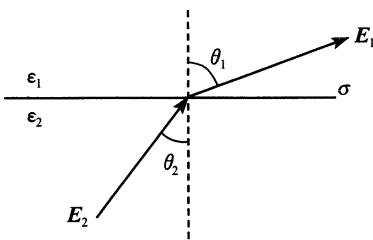
\includegraphics[width=0.3\linewidth]{figures/fig_2_19_1.jpg}
\end{center}

\vfill

\newpage

\textbf{2.19.} 如习题 2.19 图所示, 一导体球外充满两半无限电介质, 介电常量分别为 $\varepsilon_{1}$ 和 $\varepsilon_{2}$ , 介质界面为通过球心的无限平面. 设导体球半径为 $a$ , 总电荷为 $q$ , 求空间电场分布和导体球表面的自由面电荷分布.

\begin{center}
    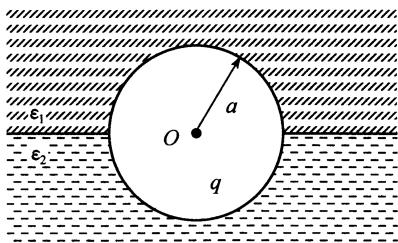
\includegraphics[width=0.3\linewidth]{figures/fig_2_19_2.jpg}
\end{center}

\vfill

\textbf{2.20.} 把平行板电容器的两极板接到电源上(接通 K)，然后在电容器内左半区中放入介电常量为 $\varepsilon$ 的电介质(见习题 2.20 图).

(1) 问 A、B 两点的场强哪个大？各为没有介质时的多少倍？

(2) 如果在充电后, 先把电源断开 (即断开 K), 再在左半区中放入介质, 电场强度如何变化?

\begin{center}
    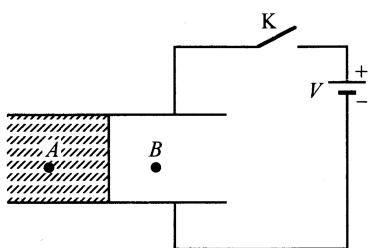
\includegraphics[width=0.3\linewidth]{figures/fig_2_20_1.jpg}
\end{center}

\vfill

\newpage

\textbf{2.21} 如习题2.21图所示, 整个空间以 $z = 0$ 为界面, 上下分别充满介电常量为 $\varepsilon_{1}$ 和 $\varepsilon_{2}$ 的介质. 在 $z = a$ 处和 $z = -a$ 处分别放置电量为 $-q$ 和 $+q$ 的点电荷, 求 $-q$ 电荷受的作用力.

\begin{center}
    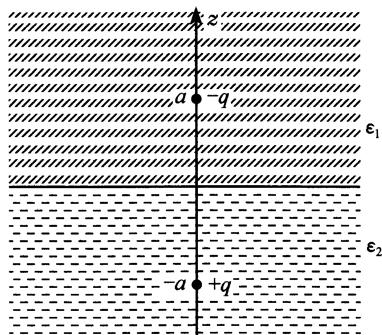
\includegraphics[width=0.3\linewidth]{figures/fig_2_20_2.jpg}
\end{center}

\vfill


\textbf{2.22.} 一电量为 $+q$ 的点电荷位于 $(x, y) = (a, b)$ ，两半无限接地导体平面相交于 $z$ 轴，如习题2.22图所示.

(1) 求 +q 所在区域 $(x, y \geqslant 0, -\infty < z < \infty)$ 中任一点的电场；

(2) 利用 $E_{y}$ 的表达式, 确定哪一个导体平板表面 $E_{y}=0$ , 并计算 $E_{y}\neq0$ 的导体平板的面电荷密度 $\sigma_{e}$ .

\begin{center}
    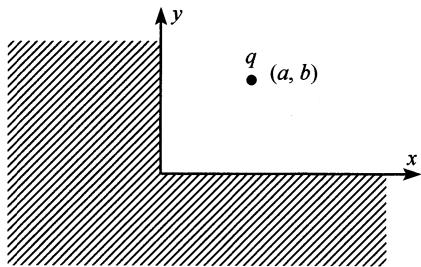
\includegraphics[width=0.4\linewidth]{figures/fig_2_22_1.jpg}
\end{center}

\vfill

\newpage

\textbf{2.23} 如习题 2.23 图所示,一半径为 $R$ 的导体球壳,球内部距离球心为 $d(d < R)$ 处有一点电荷 $q$ ,求

(1) 当球壳接地时球内的电场强度和电势；

(2) 当球壳不接地且带电量为 Q 时球内的电场强度和电势.

\begin{center}
    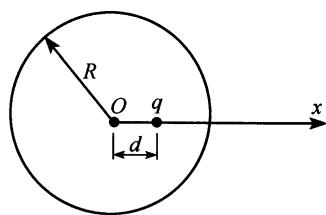
\includegraphics[width=0.3\linewidth]{figures/fig_2_22_2.jpg}
\end{center}
\vfill

\textbf{2.24} 一半径为 $a$ 的无限长的直导线的线电荷密度为 $\lambda_{\mathrm{e}}$ ，与一电势为零的无限大金属板相距为 $b, b \gg a$ ，试对单位长度导线，计算此系统的电容（提示：用电像法和条件 $b \gg a$ ）.


\vfill

\newpage
